\section{RAILS analyse} \label{app:railsAnalysis}

In deze analyse zal er worden gekeken naar welke aspecten van de soft/hardware er in de volgende ontwikkel cyclus verbeterd kunnen worden. De analyse methode die wordt gebruikt is de RAILS analyse zoals beschreven in het zesde werkcollege van het vak sensor netwerken. Een RAILS analyse bestaat uit de volgende onderdelen:
\begin{itemize}
    \item Revisie
    \item Algoritmes
    \item Interactie
    \item Lookup tabellen
    \item Slaap
\end{itemize}
De bovengenoemde onderdelen zullen in de rest van deze appendix worden beschreven.

\subsection{Revisie}

\begin{figure}[h]
    \centering
    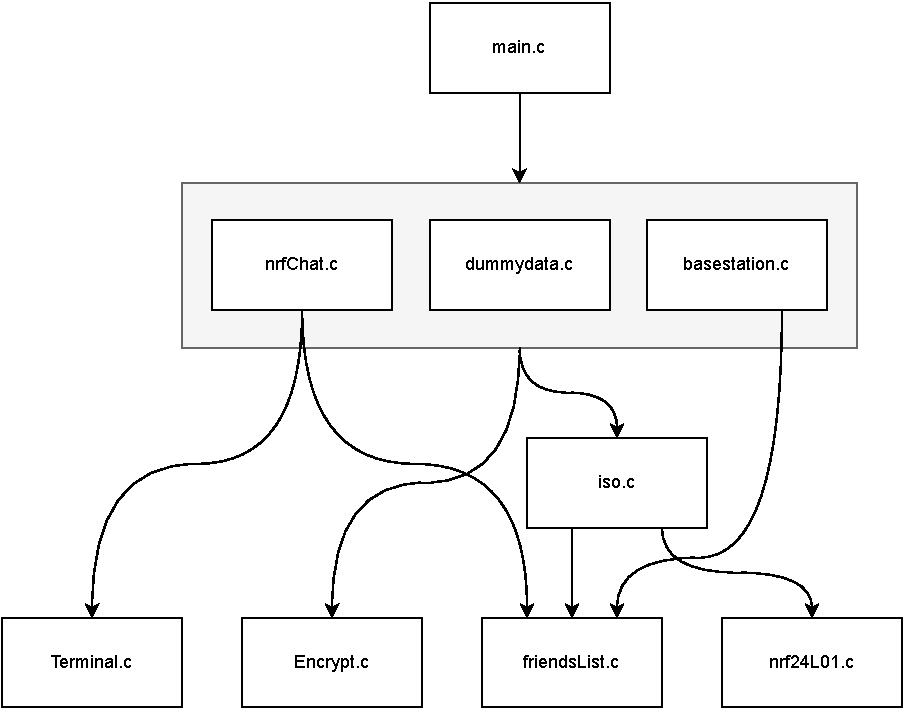
\includegraphics[width=0.6\textwidth]{img/abstractions}
\end{figure}

\subsection{Algoritmes}

% Zoek algoritme in vriendjes tabel

\subsection{Interactie}

\subsection{Lookup tabellen}

\subsection{Slaap}
% \fbox{
%     \centering
%     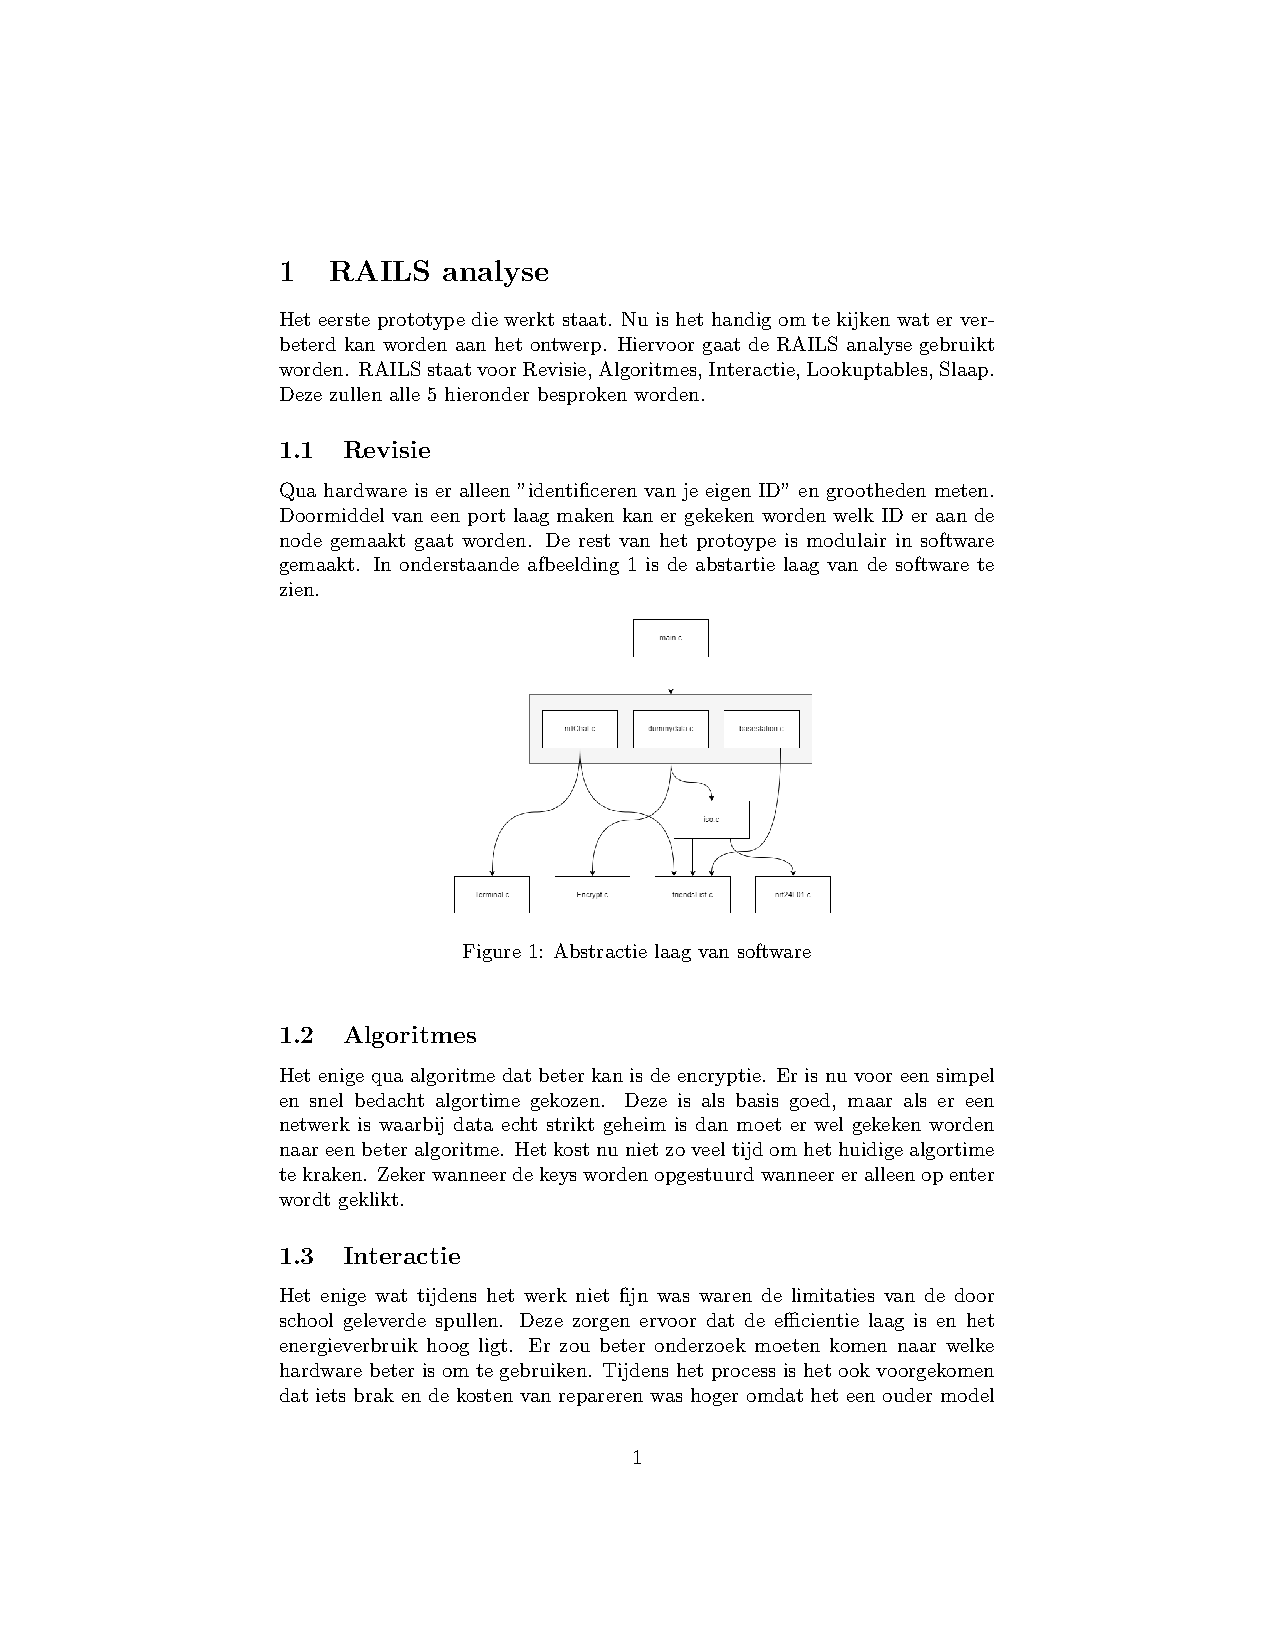
\includegraphics[page=1,scale=0.7]{img/RAILS.pdf}
% }

% \fbox{
%     \centering
%     \includegraphics[page=2,scale=0.7]{img/RAILS.pdf}
% }